\begin{frame}{Définition}
    Désigne toute transposition à l'identique ou presque d'un livre imprimé en version numérique.
    \begin{itemize}
        \item Depuis 2010 environ, souvent une version "homothétique" en plus de la version papier.
        \item 75\% du coût (environ) de la version papier.
        \item Protégés par un verrou numérique. 
    \end{itemize}

    Selon \href{https://www.unidivers.fr/livre-numerique-michel-morvan/}{Michel Morvan (professeur en informatique)}, les lecteur.rices lisent de plus en plus de numérique mais moins que sur papier.\\
    \textrightarrow{} spécificité française à cause de la loi sur le prix unique du livre, ce qui entraîne:
    \begin{itemize}
        \item Très peu de concurrence entre les librairies; 
        \item Éditeurs papiers qui publient aussi en numérique ont une politique de prix numérique élevée: rare que le livre numérique soit vendu à moins de 30 \% du prix du livre papier. 
    \end{itemize}

\end{frame}

\begin{frame}{PDF}
    \begin{columns}[T,onlytextwidth]
        \column{0.50\linewidth}
        \small
        \begin{itemize}
            \item \textit{Portable Document Format}.
            \item Présenté en 1992 par Adobe; puis devenu une norme ISO en format ouvert en 2008
            \item Premières versions ne prenaient pas en charge les hyperliens, longues à télécharger et lentes.
            \item Préservation de la mise en page d'un document telle qu'elle a été définie par son auteur.
            \item Offre une forte stabilisation.
        \end{itemize}

        \column{0.50\linewidth}
        \centering
        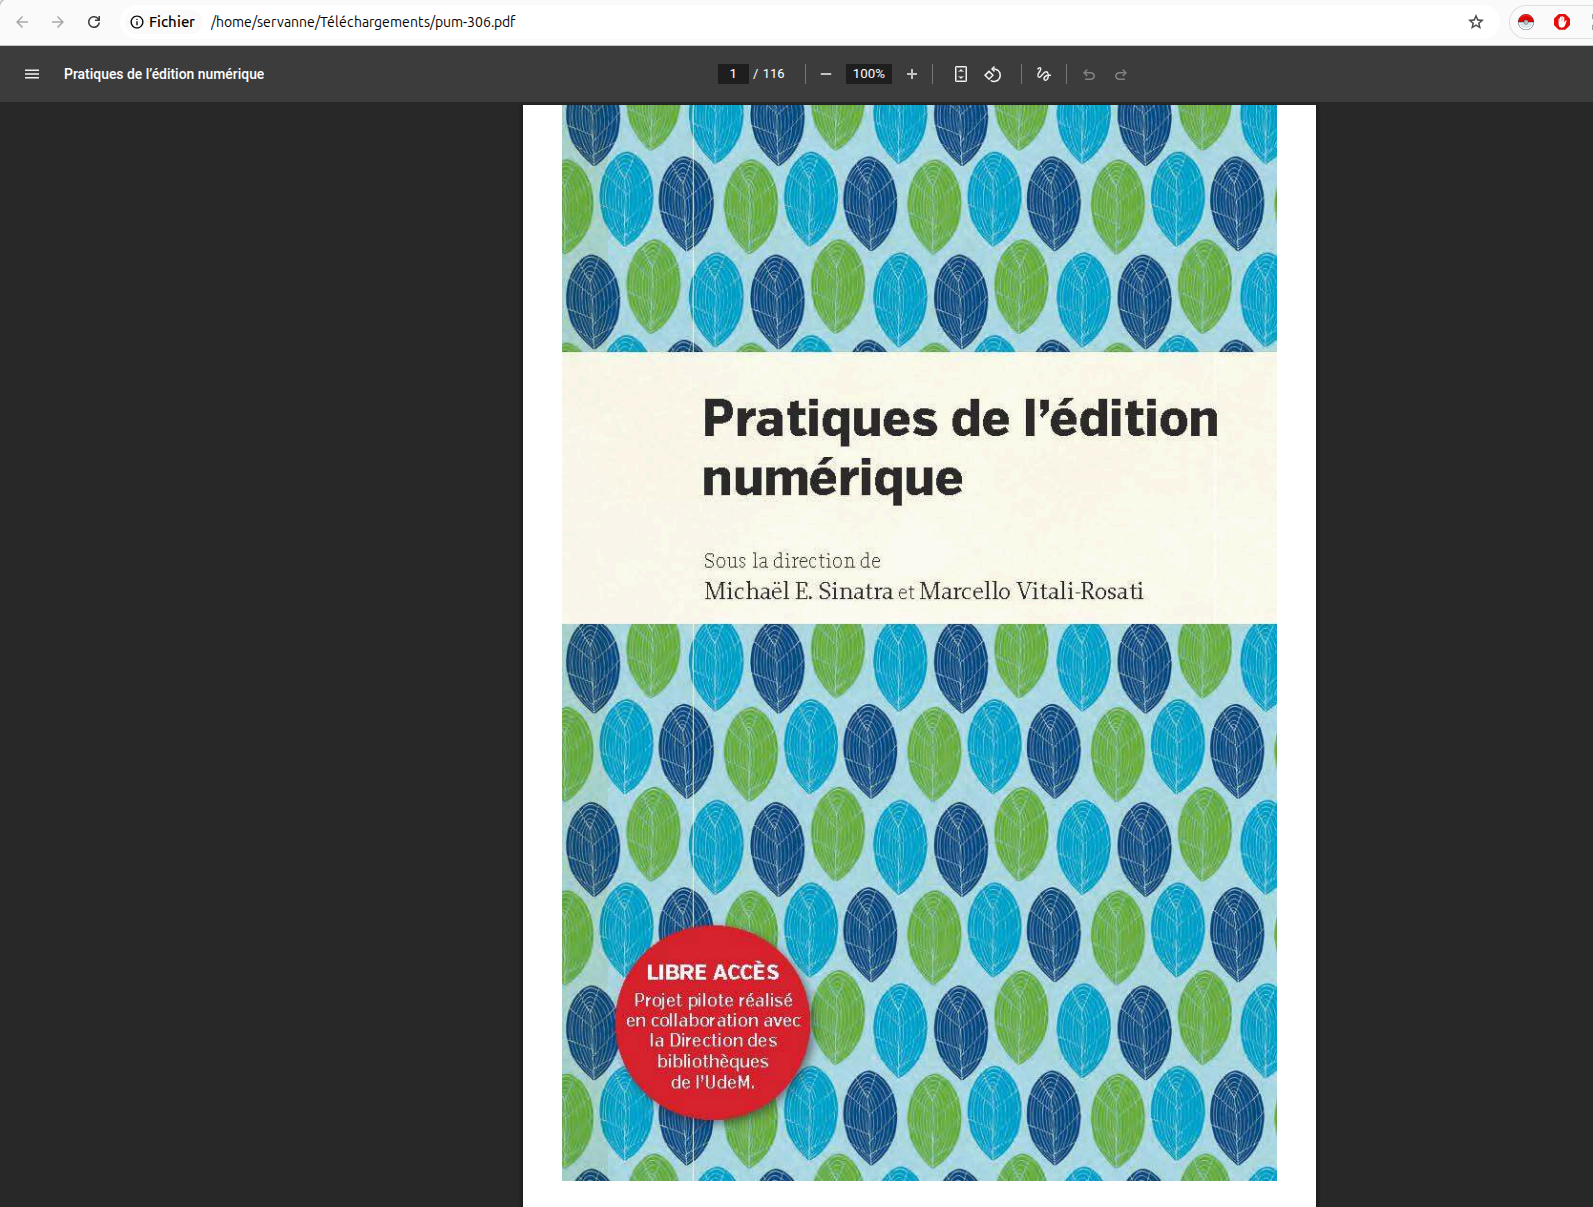
\includegraphics[width=.90\columnwidth]{Images/edition-numerique-pdf.png}
    \end{columns}
\end{frame}

\begin{frame}{PDF}
        \begin{figure}
        \centering
        \begin{subfigure}{0.4\textwidth}
            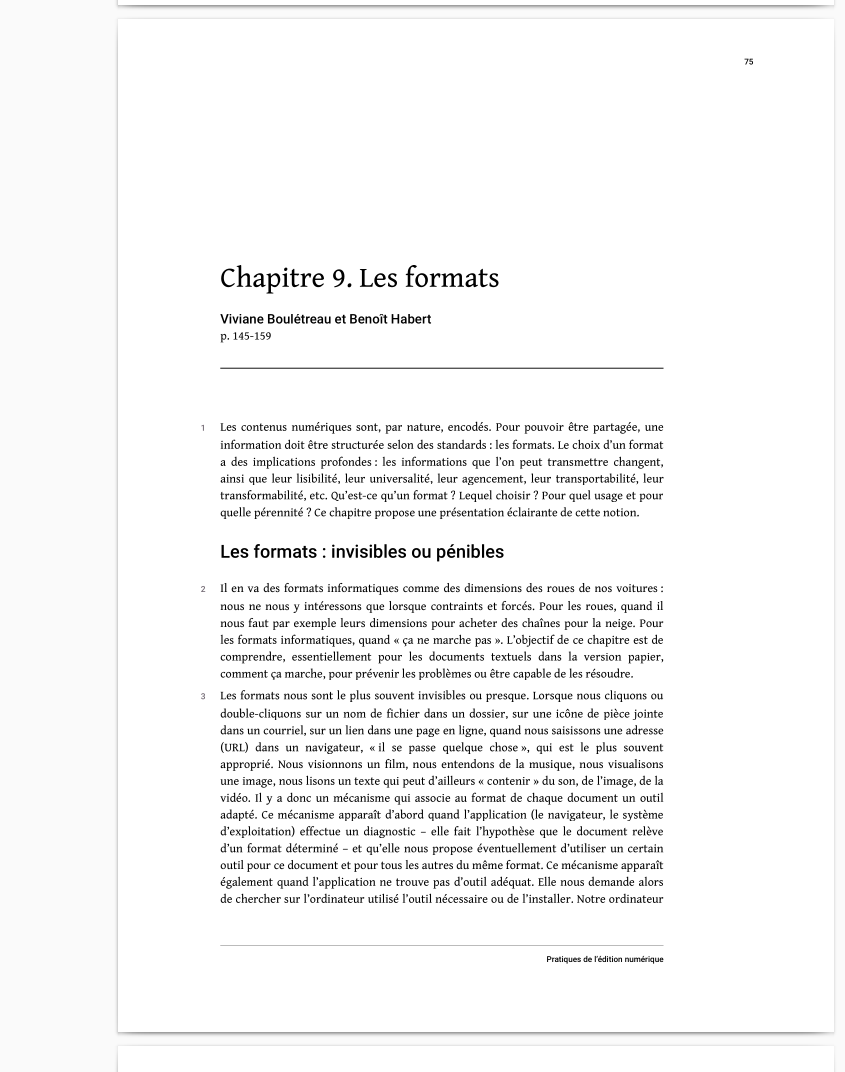
\includegraphics[height=.80\textheight,keepaspectratio]{Images/pratiques-edition-num-chap-9-pdf.png}
            \label{fig:f}  
        \end{subfigure}
        \hspace{2em}
        \begin{subfigure}{0.4\textwidth}
            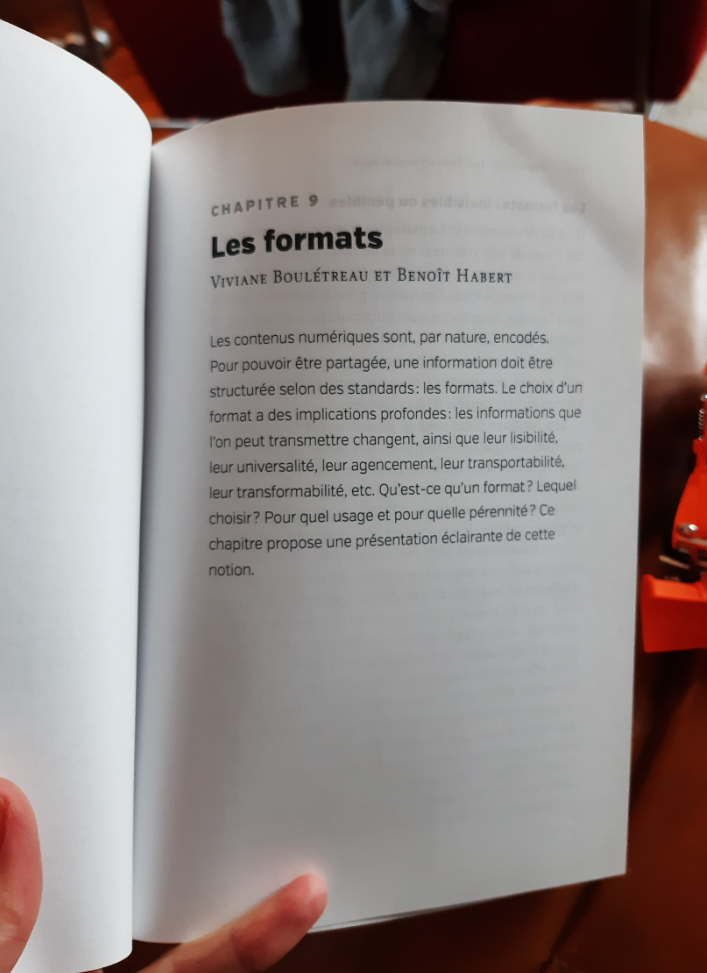
\includegraphics[height=.80\textheight, keepaspectratio]{Images/pratiques_edition_text.png}
            \label{fig:g}  
        \end{subfigure}
    \end{figure}
\end{frame}

\begin{frame}{ePUB}
    \begin{columns}[T,onlytextwidth]
        \column{0.50\linewidth}
        \small
        \begin{itemize}
            \item A pour ancêtre le format \textit{Open eBook}.
            \item Première version dans les années 2000.
            \item Format ouvert.
            \item Conçu pour faciliter la mise en page du contenu: fluide et s'adapte facilement à l'écran de lecture.
        \end{itemize}

        \column{0.50\linewidth}
        \centering
        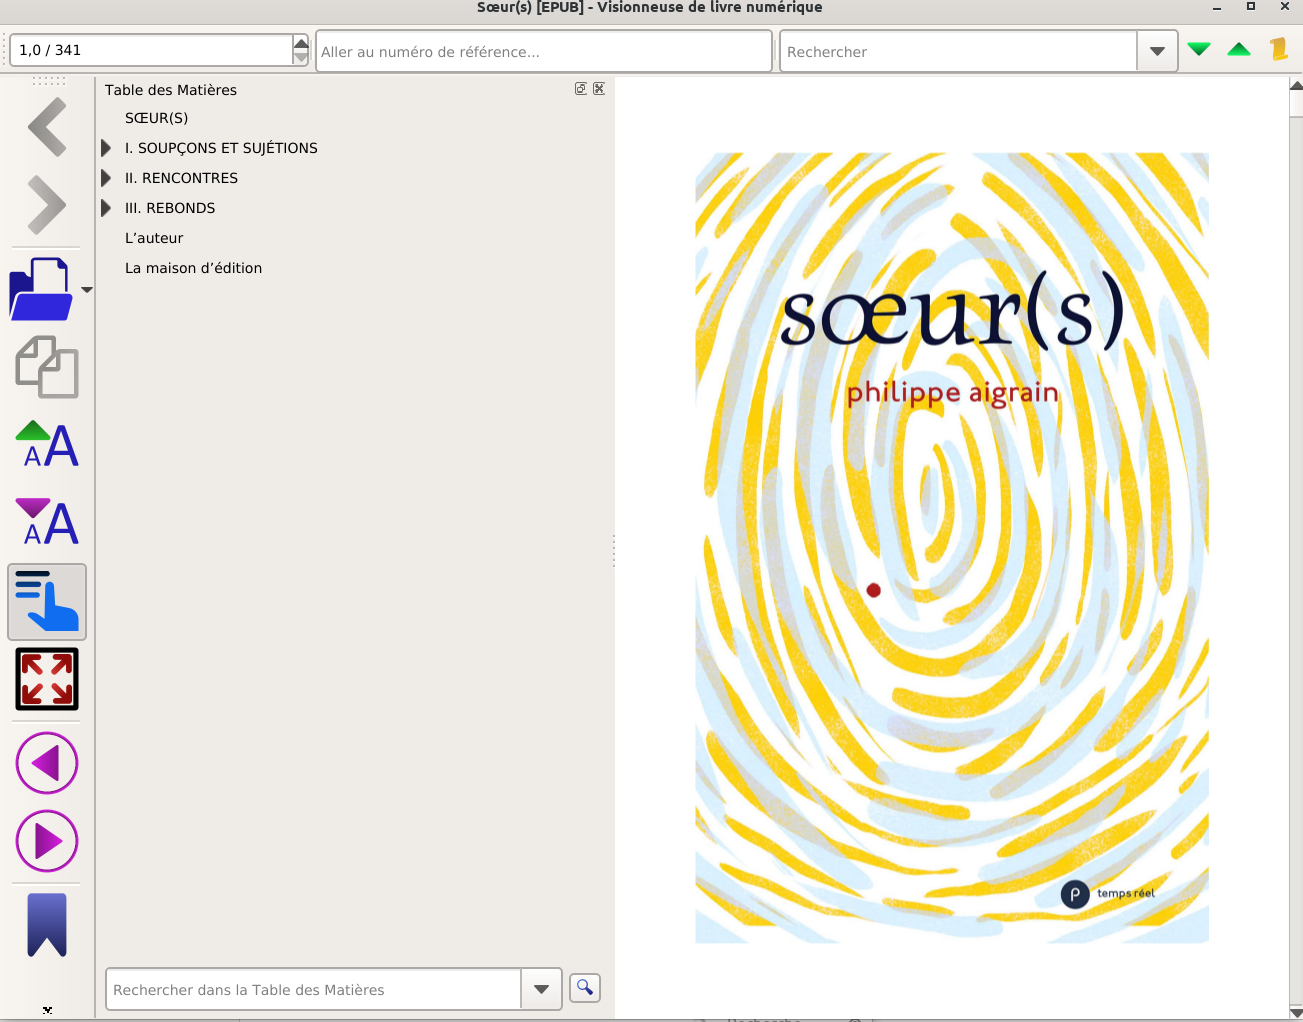
\includegraphics[width=.90\columnwidth]{Images/epub1.png}
    \end{columns}
\end{frame}

\begin{frame}{AZW (Kindle)}
    \begin{columns}[T,onlytextwidth]
        \column{0.50\linewidth}
        \small
        \begin{itemize}
            \item Format propriétaire.
            \item A développé le modèle économique d'Amazon: ne pas vendre des livres mais l'accès à un catalogue.
            \item Première liseuse en 2007.
            \item Conçu pour faciliter la mise en page du contenu: fluide et s'adapte facilement à l'écran de lecture.
        \end{itemize}

        \column{0.50\linewidth}
        \centering
        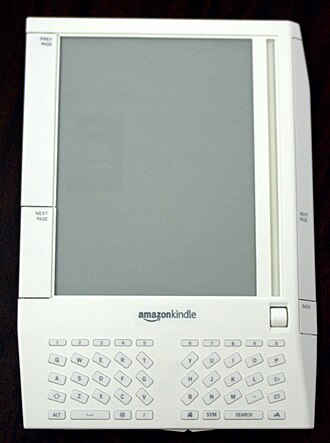
\includegraphics[width=.90\columnwidth]{Images/Amazon_Kindle_-_Off.jpg}
    \end{columns}
    
\end{frame}

\begin{frame}{AZW (Kindle)}
    \centering
    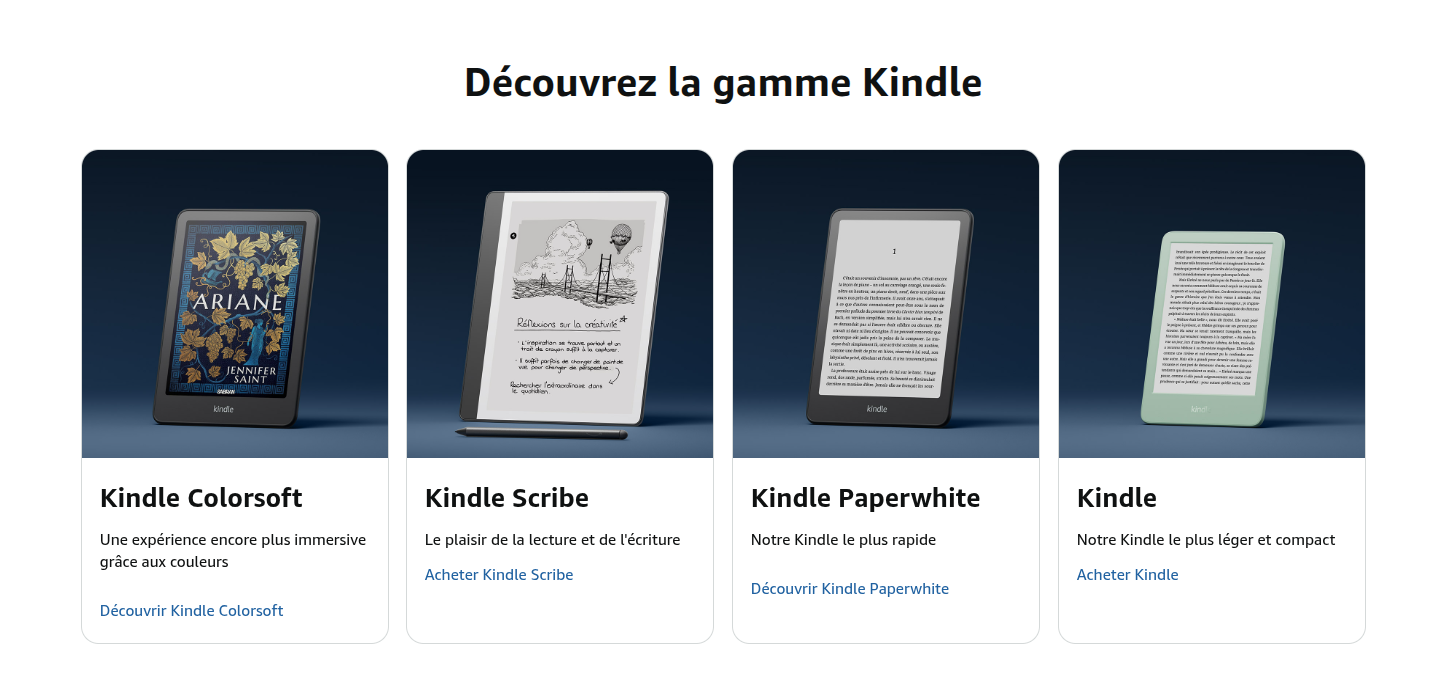
\includegraphics[width=\textwidth]{Images/kindle-gamme.png}
\end{frame}